
% Outline: 28 Jan 2019
%   - 0. Summary (PAPPG guidlines) - 1p
%   - 1. Project Description - 10 pp
%   - 1.1 Intellectual Merit:
%       - 1.1.1 Background \& Motivation
%           - LSST cost NSF ~ \$1B
%               - LSST Science goals
%           - Can think of LSST as the next generation SDSS
%               - But it doesn't have spectroscopy!
%           - SDSS was an Imaging + Spectroscopy survey
%               - SDSS the most cited survey ever
%               - SDSS science milestones
%               - Spectroscopy was a key aspect for the success of SDSS
%                 (MPA-JHU)
%               - Public release of data also key
%           - What would it look like to perform SDSS-like spectroscopy
%             for the LSST imagine survey?
%               - Fraction of observed objects
%               - Cost
%               - currently an intractible problem
%                   - link to photonics development?
%               - Need new techniques (machine learning) to infer
%                 statistically accurate population characteristics with
%                 small training sets
%           - LSST Science themes
%           - Science enabled by LSST spectroscopy, lay groundwork for
%             later science discussion.
%
%       - 1.1.2 Research Community Priority
%           - Review Astro2010
%               - LSST
%           - Preview of or predictions for astro2020
%           - Big data initiatives:
%               - Moore-Sloan Data-Science Environments
%                   - Berkeley institute for data science, NYU, UW
%               - Using subsets of training data to understand a
%                 population
%                   - Hogg's AAS talk...
%
%           - Spectroscopy of LSST sources to get photozs provides key
%             advantages to Cosmology/Dark Energy
%           - Time domain astrophysics
%               - AGN, CVs, stars (astroseismology)
%
%       - 1.1.3 Astrophysics and Data Science Goals
%           - A Universe in transition
%               - Gravity to Dark Energy:
%                   - Precise cosmology with LSST and trained photozs
%               - Gas to stellar dominated: The Galactic Ecosystem at z~2
%                   - environment (Cooper)
%                   - absorption-line systems (Prochaska)
%                   - stellar populations (Shapely, Siana)
%                       - Bootstrap z~2 properties to higher redshift (z~7)
%               - Neutral to ionized gas: The heterogeneity of
%                 Reionization
%                   - environment and neutral fractions (Becker)
%                   - Ly continuum (photon budget) at z~5-7 (Siana)
%           - The Chemodynamical history of the Local Group
%               - Chemical tagging of GAIA spectra on the far side of
%                 the Milky Way (Yuan-Sen)
%                   - What's gained in 0.31-0.4 range (unavailable to
%                     PFS)
%               - MW/M31/M33 (Raja, Connie)
%               - Life cycle of stellar clusters
%           - Time Domain (Foley)
%
%       - 1.1.4 FOBOS
%           - How does FOBOS meet the science goals?
%           - Instrument description as of conceptual design
%           - Development from concept to final design
%               - Sketch of timeline
%           - Public survey design
%               - Key science programs
%               - AI-informed targeting system
%               - Robust DRP and DAP
%               - Public release schedule
%           - Longer-term strategy for public release of *any* FOBOS
%             data
%               - 18-month proprietary period for PI data
%               - Observatory queue for opportunistic use of "free"
%                 fibers
%
%       - 1.2 Broader Impacts
%           - Student Training
%           - ISEE, AKAMAI (Lisa Hunter)
%           - New UCSC Astrophysics major with Data Science emphasis
%               - New course, summer projects
%   
%   - 2. References (2-page max)
%
%   - 3. Biographical Sketches (2 pages each), required for PI, co-PIs,
%     and any additional senior personnel (see PAPPG)
%
%   - 4. Budget and Budget Justification: "For preliminary proposals
%     cost estimates may be preliminary estimates with the Basis of
%     Estimates (BoE) included. Copies of vendor quotations should not
%     be included in preliminary proposals. If the budget includes
%     contingency, that contingency should cover the 'known unknowns'
%     and be used to mitigate identified risks."
%
%   - 5. Facilities, Equipment, and Other Resources: "In order for NSF,
%     and its reviewers, to assess the scope of a proposed project, all
%     organizational resources necessary for, and available to a
%     project, must be described in this section of the proposal.
%     Proposers should describe only those resources that are directly
%     applicable. The description should be narrative in nature and must
%     not include any quantifiable financial information. Proposers
%     should include a description of the internal and external
%     resources (both physical and personnel) that are expected to be
%     available to the project.  Such information must be provided in
%     this section, in lieu of other parts of the proposal (e.g., Budget
%     Justification, Project Description)."
%
%   - 6. Supplementary Documents:
%           - A list of the major team members, their affiliations, and
%             their role in the project
%           - A list of Partner Organizations to be funded via
%             subawards, and the role of each in the project
%           - An outline of the Project Execution Plan (PEP) . See the
%             LFM/MFG. Greater detail will be required in invited full
%             proposals should that occur.
%
%         "No other items or appendices should be included. Information
%         pertaining to 'Results from Prior NSF Support', 'Current and
%         Pending Support', 'Data Management Plan', and 'Postdoctoral
%         Mentoring Plan' is not required for preliminary proposals and
%         should not be included. Preliminary proposals containing items
%         other than those required above will be returned without
%         review.


%\documentclass[11pt,letterpaper]{article}
\documentclass[oneside,11pt]{amsart}

%\usepackage{a4wide}
%\usepackage{epsfig}
%\usepackage{psfig}
\usepackage{graphicx}
\usepackage{natbib,latexsym,url,enumitem,pdfpages}
\usepackage{color}
\usepackage{wrapfig}

% Some fancy commenting
\definecolor{todo}{RGB}{200,0,0}
\newcommand{\comment}[2][todo]{{\color{#1}[[{\bf #2}]]}}

% User commands
\makeatletter
\let\jnl@style=\rm
\def\ref@jnl#1{{\jnl@style#1}}

\def\ref@jnl#1{{\jnl@style#1}}% 
\newcommand\aj{\ref@jnl{AJ}}%        % Astronomical Journal 
\newcommand\araa{\ref@jnl{ARA\&A}}%  % Annual Review of Astron and Astrophys 
\newcommand\apj{\ref@jnl{ApJ}}%    % Astrophysical Journal ++
\newcommand\apjl{\ref@jnl{ApJL}}     % Astrophysical Journal, Letters 
\newcommand\apjs{\ref@jnl{ApJS}}%    % Astrophysical Journal, Supplement 
\newcommand\ao{\ref@jnl{ApOpt}}%   % Applied Optics ++
\newcommand\apss{\ref@jnl{Ap\&SS}}%  % Astrophysics and Space Science 
\newcommand\aap{\ref@jnl{A\&A}}%     % Astronomy and Astrophysics 
\newcommand\aapr{\ref@jnl{A\&A~Rv}}%  % Astronomy and Astrophysics Reviews 
\newcommand\aaps{\ref@jnl{A\&AS}}%    % Astronomy and Astrophysics, Supplement 
\newcommand\azh{\ref@jnl{AZh}}%       % Astronomicheskii Zhurnal 
\newcommand\baas{\ref@jnl{BAAS}}%     % Bulletin of the AAS 
\newcommand\icarus{\ref@jnl{Icarus}}% % Icarus
\newcommand\jrasc{\ref@jnl{JRASC}}%   % Journal of the RAS of Canada 
\newcommand\memras{\ref@jnl{MmRAS}}%  % Memoirs of the RAS 
\newcommand\mnras{\ref@jnl{MNRAS}}%   % Monthly Notices of the RAS 
\newcommand\pra{\ref@jnl{PhRvA}}% % Physical Review A: General Physics ++
\newcommand\prb{\ref@jnl{PhRvB}}% % Physical Review B: Solid State ++
\newcommand\prc{\ref@jnl{PhRvC}}% % Physical Review C ++
\newcommand\prd{\ref@jnl{PhRvD}}% % Physical Review D ++
\newcommand\pre{\ref@jnl{PhRvE}}% % Physical Review E ++
\newcommand\prl{\ref@jnl{PhRvL}}% % Physical Review Letters 
\newcommand\pasp{\ref@jnl{PASP}}%     % Publications of the ASP 
\newcommand\pasj{\ref@jnl{PASJ}}%     % Publications of the ASJ 
\newcommand\qjras{\ref@jnl{QJRAS}}%   % Quarterly Journal of the RAS 
\newcommand\skytel{\ref@jnl{S\&T}}%   % Sky and Telescope 
\newcommand\solphys{\ref@jnl{SoPh}}% % Solar Physics 
\newcommand\sovast{\ref@jnl{Soviet~Ast.}}% % Soviet Astronomy 
\newcommand\ssr{\ref@jnl{SSRv}}% % Space Science Reviews 
\newcommand\zap{\ref@jnl{ZA}}%       % Zeitschrift fuer Astrophysik 
\newcommand\nat{\ref@jnl{Nature}}%  % Nature 
\newcommand\iaucirc{\ref@jnl{IAUC}}% % IAU Cirulars 
\newcommand\aplett{\ref@jnl{Astrophys.~Lett.}}%  % Astrophysics Letters 
\newcommand\apspr{\ref@jnl{Astrophys.~Space~Phys.~Res.}}% % Astrophysics Space Physics Research 
\newcommand\bain{\ref@jnl{BAN}}% % Bulletin Astronomical Institute of the Netherlands 
\newcommand\fcp{\ref@jnl{FCPh}}%   % Fundamental Cosmic Physics 
\newcommand\gca{\ref@jnl{GeoCoA}}% % Geochimica Cosmochimica Acta 
\newcommand\grl{\ref@jnl{Geophys.~Res.~Lett.}}%  % Geophysics Research Letters 
\newcommand\jcp{\ref@jnl{JChPh}}%     % Journal of Chemical Physics 
\newcommand\jgr{\ref@jnl{J.~Geophys.~Res.}}%     % Journal of Geophysics Research 
\newcommand\jqsrt{\ref@jnl{JQSRT}}%   % Journal of Quantitiative Spectroscopy and Radiative Trasfer 
\newcommand\memsai{\ref@jnl{MmSAI}}% % Mem. Societa Astronomica Italiana 
\newcommand\nphysa{\ref@jnl{NuPhA}}%     % Nuclear Physics A 
\newcommand\physrep{\ref@jnl{PhR}}%       % Physics Reports 
\newcommand\physscr{\ref@jnl{PhyS}}%        % Physica Scripta 
\newcommand\planss{\ref@jnl{Planet.~Space~Sci.}}%  % Planetary Space Science 
\newcommand\procspie{\ref@jnl{Proc.~SPIE}}%      % Proceedings of the SPIE 

\newcommand\actaa{\ref@jnl{AcA}}%  % Acta Astronomica
\newcommand\caa{\ref@jnl{ChA\&A}}%  % Chinese Astronomy and Astrophysics
\newcommand\cjaa{\ref@jnl{ChJA\&A}}%  % Chinese Journal of Astronomy and Astrophysics
\newcommand\jcap{\ref@jnl{JCAP}}%  % Journal of Cosmology and Astroparticle Physics
\newcommand\na{\ref@jnl{NewA}}%  % New Astronomy
\newcommand\nar{\ref@jnl{NewAR}}%  % New Astronomy Review
\newcommand\pasa{\ref@jnl{PASA}}%  % Publications of the Astron. Soc. of Australia
\newcommand\rmxaa{\ref@jnl{RMxAA}}%  % Revista Mexicana de Astronomia y Astrofisica

%% added feb 9, 2016
\newcommand\maps{\ref@jnl{M\&PS}}% Meteoritics and Planetary Science
\newcommand\aas{\ref@jnl{AAS Meeting Abstracts}}% American Astronomical Society Meeting Abstracts
\newcommand\dps{\ref@jnl{AAS/DPS Meeting Abstracts}}% American Astronomical Society/Division for Planetary Sciences Meeting Abstracts



\let\astap=\aap 
\let\apjlett=\apjl 
\let\apjsupp=\apjs 
\let\applopt=\ao 



\DeclareRobustCommand{\gtrsim}{%
\mathrel{\hskip-.5em\begin{array}{c}>\\[-8pt]\sim\end{array}\hskip-.5em}}
\DeclareRobustCommand{\lesssim}{%
\mathrel{\hskip-.5em\begin{array}{c}<\\[-8pt]\sim\end{array}\hskip-.5em}}

\pretolerance=10000
\textwidth=6.4in
\textheight=8.95in
\voffset = 0.in
%\voffset = -0.3in  % For my printer
\topmargin=0.0in
\headheight=0.00in
\hoffset = 0.0in
%\hoffset = 0.33in  %  For my printer
\headsep=0.00in
\oddsidemargin=0in
\evensidemargin=0in
\parindent=2em
\parskip=0.2ex
 
\renewcommand{\baselinestretch}{1.03}

\special{papersize=8.5in,11in}



\setlength{\parskip}{0.6 ex plus 0.4ex minus 0.2ex} \flushbottom
\pagestyle{plain} 

\begin{document}
% \thispagestyle{empty}

\pagenumbering{arabic}
\begin{center}

\vspace*{-1.5cm}

%\textbf{\textsf{Training LSST with Keck-FOBOS:\\ Comprehensive, Data-Driven Models of a Universe in Transition}}
\textbf{\textsf{Training Imaging Surveys with Deep Spectroscopy:\\ Comprehensive, Data-Driven Models of a Universe in Transition}}

\authors{K. Bundy, K. Westfall, N. MacDonald, P. Capak, A. Coil, C. Conroy, M. Cooper, R. Kupke, K.G. Lee, R.
Mandelbaum, D. Masters, J. Newman, X. Prochaska, C. Rockosi, J. Rhodes, M. Rich, M. Savage, A. Shapley, B. Siana, Y.-S.
Ting}

\end{center}

\noindent\comment{10-page limit, excluding references.  This Mid-scale Research Infrastructure-1 ``Design'' proposal
requests funds to complete the preliminary instrument design for the Fiber-Optic Broadband Optical Spectrograph
(FOBOS) and build frameworks for enabling data-driven science goals via a FOBOS Public Survey.}


% \smallskip
% \section{Project Summary}
% \label{sec:summary}

% \noindent\comment{1 pg, doesn't count towards 10-pg limit}

% \noindent {\bf Overview:}
% (activity that would result and methods)

% \noindent {\bf Intellectural Merit:}

% \noindent {\bf Broader Impacts:}

% \clearpage


\smallskip
\section{Intellectual Merit}
\label{sec:im}

\subsection{Scientific Justification} 
\noindent \comment{3/4 page}

% "including the unique research
% capabilities and lack of general availability of the requested
% infrastructure and its potential to significantly advance the Nation’s
% research infrastructure."


Led by NSF's Large Synoptic Survey Telescope (LSST) which deploys in 2023, astronomy is entering a new era of
unprecedented deep-imaging data sets that will survey huge volumes of the universe when it was only one-half or
one-third its current age.  These epochs mark important but poorly understood transitions in cosmic history. Early
galaxies were emerging from a ``primordial soup'' of gas and dust, assembling now fossilized structures that may be
detected even within our own Milky Way.  Meanwhile, the rate of cosmic expansion was beginning to accelerate, as the
Universe became increasingly dominated by ``Dark Energy,'' whose origin remains the single greatest mystery in
astronomy and cosmology today.

Since Edwin Hubble's observations over 100 years ago, major advances in our understanding of the universe have come
from the two-step process of first taking images of the sky to locate sources of interest and then obtaining
information-rich spectroscopy to reveal the nature of those sources.  A modern example is the Sloan Digital Sky Survey
(SDSS) whose combination of panoramic ``imaging'' followed by dedicated spectroscopy yielded an unprecedented sample of
over 1 million galaxies, mapping the present-day universe and making SDSS the most highly cited survey in the history
of astronomy.

% Because a quality spectrum requires far more observing time per source than an image, SDSS pioneered ``high multiplex''
% spectrographs, capable of \emph{simultaneous} spectroscopy of hundreds of objects.

LSST's all-sky images will be 1,000 times deeper and detect far more distant galaxies than SDSS, but {\bf no current
U.S. facility is capable obtainng the spectroscopic followup} at a level required to capitalize on our \$1B investment
in LSST.  In fact, SDSS-like spectroscopic followup of 1 million galaxies at LSST distances would require 300 years of
observing on the largest telescopes with current instrumentation!

The only way forward is encapsulated in one of NSF's ``10 Big Ideas,'' namely \emph{Harnessing the Data Revolution} in
order to maximize the information content of LSST via machine learning of optimally-designed spectroscopic training
sets.  This proposal presents a connected approach to the three critical components in this endeavor: 1) Development of
statistical approaches to specific and ambitious data-science challenges that will address key questions about
transitional epochs in cosmic history; 2) Design of FOBOS, a state-of-the-art spectroscopic facility on one of the
world's largest telescopes optimized for obtaining spectroscopic training sets; 3) Design and execution
of a ``Public Survey'' with this facility as well as a data-serving platform to provide spectroscopy and training data
to the U.S. community.  This MSRI-1 design proposal lays out the path for maximizing the panoramic imaging of LSST with
spectroscopic followup.  Through a subsequent MSRI proposal we will deliver on our goals with an instrument deployment
in 2026 and completed spectroscopic followup as LSST concludes in 2029.

We address data science challenges in four research areas in order to guide our instrument and survey design:

\begin{enumerate}
	\item Significantly more powerful probes of Dark Energy and Cosmology
	\item Comprehensive understanding of the proto-galaxy ecosystem at $z\sim2$
	\item Archaeological studies of our own Milky Way galaxy and its satellites to unravel their specific journeys
	through this transition.
	\item Time domain spectroscopy...?
\end{enumerate}


% Reference test: \citet{2015ApJ...798....7B}.



\subsection{Research Community Priority} 
\label{sec:community}
\noindent\comment{3/4 page}

% \noindent "evidence, such as workshop
% reports or other publicly available indicators, that the infrastructure
% is a priority for a research community or important for a recognized NSF
% priority area such as one of NSF’s research Big Ideas."

% The coming decade will benefit from  major investments in both the depth and breadth of astronomical observations.  The James Webb Space Telescope will provide our deepest views yet, probing the first billion years of cosmic time over narrow sightlines.  At the same time, LSST's panoramic imaging will survey broad cosmic volumes of unprecedented size, detecting the majority of luminous sources a few billion years later.  LSST's optical imaging will be complemented by space-based near-infrared imaging from Euclid and eventually's NASA's WFIRST. 

The need for spectroscopic followup in the LSST era was made clear in the National Research Council's 2015 report, ``Optimizing the U.S. Ground-Based Optical and Infrared Astronomy System'' \citep{NAP21722} which made the following recommendation:

\begin{quote}
The National Science Foundation should support the development of a wide-field, highly multiplexed spectroscopic capability on a medium- or large-aperture telescope in the Southern Hemisphere to enable a wide variety of science, including follow-up spectroscopy of Large Synoptic Survey Telescope targets. Examples of enabled science are studies of cosmology, galaxy evolution, quasars, and the Milky Way.
\end{quote}

% \begin{quote}
% The science reach of LSST could be substantially enhanced by developing for the U.S. astronomy community a very-wide-field, massively multiplexed, spectroscopic capability. This facility should be capable of overlapping the majority of the sky area covered by the LSST surveys. Such a wide-field instrument or instruments should be sufficiently multiplexed to enable spectroscopic surveys of tens of millions of objects over several years. The science case for such a capability is rich for objects of a wide range of brightnesses...
% \end{quote}

% Therefore MSE as currently envisioned:  (https://www.noao.edu/meetings/2020decadal/files/PHall_MSE_Tucson_201802v3.pdf)
% •  will have access to 74% of the primary LSST footprint
% •  will meet its science requirements over 59% of the primary
% LSST area
% •  will observe at airmass < 1.4 (the LSST limit in its primary
% footprint) over 51% of the primary LSST area.

In addition to this report, further details of spectroscopic needs for LSST in all science areas were disseminated
after a 2013 workshop on this topic organized by the National Optical
Astronomy Observatory (NOAO).  Based on these recommendations, we propose the Keck-FOBOS instrument coupled
with a suite of data-driven tools to address LSST's spectroscopic requirements at a final cost 20 times less than
a new Southern Hemisphere facility. Located in Hawaii, Keck-FOBOS would have access to greater than 70\% of the LSST
footprint, more than adequate for our primary goal of building powerful spectroscopic training sets.  FOBOS would complement future ambitious facilities that could cover wider areas (several deg$^2$ per pointing) at shallower depths.

The need for deep spectroscopic followup is particularly acute for LSST's major cosmological probes which rely on ``photometric redshifts.''  \citet{newman15} summarize the case and describe a redshift survey which, if carried out with Keck-FOBOS, would increase LSST's Dark Energy Figure-of-Merit by a factor of 50\% at a cost of less than 5\% of the LSST budget.  The urgent case for spectroscopic redshift training has been the subject of numerous publications \citep[e.g.,][]{laureijs11,masters15, hemmati18}.  

Meanwhile, the astronomy community recognizes that the coming era of ``Big Data'' astronomy culminating in LSST
necessitates ``harnessing the data revolution.  Wide-spread community interest in advanced data science techniques
continues to grow amidst calls for educational structures, conference series, and research funding to support the
growth of a new field, ``Astroinformatics,'' which exploits the interface between astrophysics and statistics
\citep{borne09}.  Astronomy's largest organizations, including the American Astronomical Society and the International
Astronomical Union, have supported active working groups on astroinformatics and astrostatistics since 2015.  LSST
itself has built the Informatics and Statistics Science Collaboration and partnered with NSF to fund the Data Science
Fellowship Program to train astronomy graduate students in data science techniques.  Our proposal builds on and
contributes to these ongoing efforts.

% The coming decade will benefit from  major investments in both the depth and breadth of astronomical observations.  The
% James Webb Space Telescope will provide our deepest views yet, probing the first billion years of cosmic time over
% narrow sightlines.  At the same time, LSST's panoramic imaging will survey broad cosmic volumes of unprecedented size,
% detecting the majority of luminous sources a few billion years later.  LSST's optical imaging will be complemented by
% space-based near-infrared imaging from Euclid and eventually's NASA's WFIRST.

% The lack of telescope facilities capable of providing required spectrocopic followup for LSST, Euclid, and WFIRST is an urgent problem.  


\subsection{Data-Driven Science Challenges}
\label{sec:goals}

We introduce data science challenges in three science areas that will be addressed in this proposal.  Each enables significant advances in our understanding of transitional epochs in cosmic history by leveraging FOBOS-derived spectroscopic training sets to maximize the information that can be extracted from LSST.

\subsubsection{Enhancing Dark Energy Probes via Precision Cosmic Distances}
\label{sec:cosmology}
\noindent \comment{1 page}


\begin{figure}[h!]
 \vskip -0.1in
 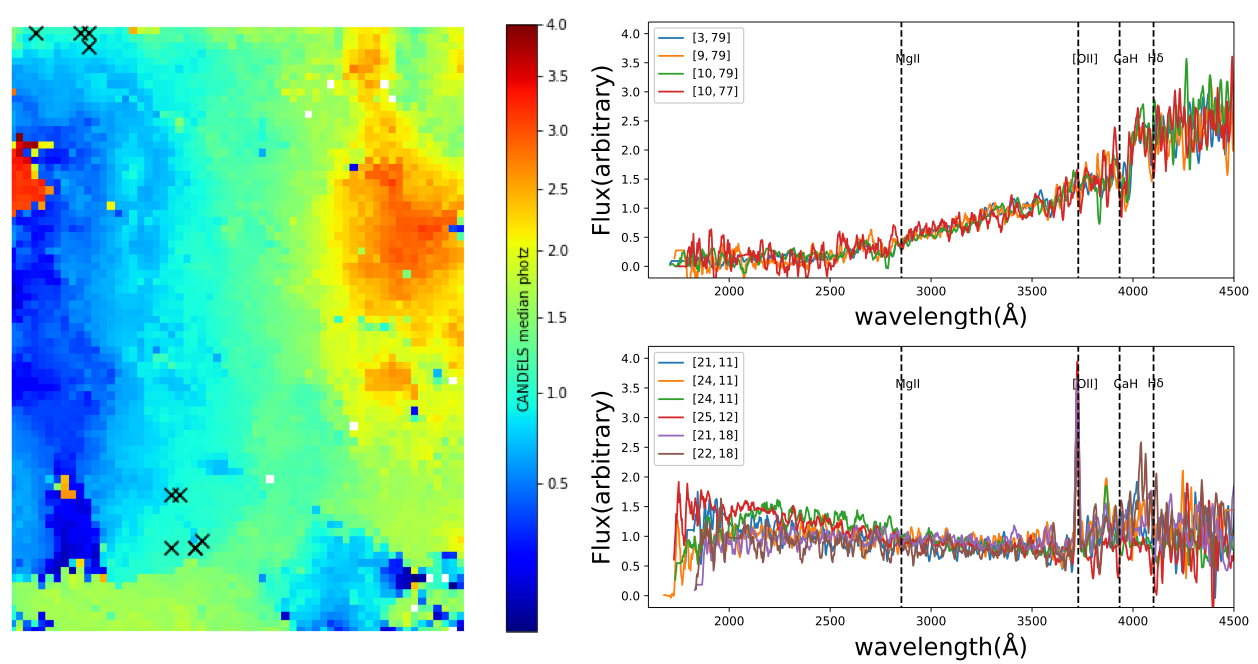
\includegraphics[width=\textwidth]{Hemmati18_Fig8_VVDS_spec.png}
 \caption{\small \emph{Left:} A Self-Organizing Map (SOM) from \citet{hemmati18} visualizing the relationship between
 broadband galaxy brightness in different broadband filters (projected along the x and y axes) and observed
 spectroscopic redshift (indicated by the color map).  SOMs guide the optimal construction of training samples by
 highlighting which galaxy classes require targeting.  \emph{Right:} Remarkably, the spectra associated with localized
 SOM regions are surprisingly similar, not just the associated redshifts.}\label{fig:SOM}
\end{figure}

The 2011 Nobel Prize in Physics was awarded for the discovery of an era of acceleration in the expansion rate of the
universe that sets in when the universe was roughly half its current age.  This accelerated expansion is often
attributed to a mysterious ``Dark Energy,'' but the amplitude of this vacuum energy density is 120 orders of magnitude
smaller than what naive models would predict.

Dark Energy is perhaps the single most important unsolved problem in cosmology and astrophysics.  As such, it has
inspired enormous world-wide effort and the construction of dedicated ground and space-based facilities.  These include
LSST, Euclid, and WFIRST.  The goal of these experiments is the precision mapping of cosmic structure.  Because this
structure expands as the universe expands, precise measures of cosmic structure allow us to reconstruct the cosmic
expansion history, and at sufficient levels of detail, distinguish among various Dark Energy models.

Many of the most important cosmological probes require galaxy ``redshifts,'' a Doppler-like shift in the observed
wavelengths of emitted light, as distant galaxies appear to recede from us as a result of cosmic expansion.
Cosmological models, which provide access to Dark Energy parameters, are constrained in part via the conversion of
redshift into distance.  Accurate redshifts are conventionally derived via spectroscopy by fitting the observed
wavelength locations of spectral features.  Less precise redshifts, so-called ``photometric redshifts'' (or photo-$z$s) can be estimated with imaging photometry alone, a
compelling option for large and faint data sets where spectroscopic redshifts are infeasible.  But, ``to infer
cosmological parameters not limited by systematic errors, accurate redshift measurements are needed'' \citep
{hemmati18}.  

Spectroscopic redshifts are critical for both the training of photometric redshift algorithms and for calibrating
results in order to correct for biases.  Complete photo-$z$ training samples can \emph{increase the Dark Energy
Figure of Merit in LSST by 50\%} \citep{newman15}.  

\medskip
\noindent {\bf Data Science Challenge 1: Obtain precise LSST Photometric Redshifts ($\sigma_z/(1+z) \lesssim 0.005$ at
i(AB) $<$ 25.3) with Targeted Training Sample sizes of $<$10k}.  Our proposed FOBOS instrument is ideally suited to
providing the spectroscopic training defined in \citet{newman15}, but a complete program would require a 400-night
investment in 10 m telescope time.  This challenge demands a reduction in the required FOBOS training sample by a
factor of $\sim$4 via clever application of state-of-the-art machine learning techniques.

Neural network trained photo-$z$s have long been recognized for providing the best precision when sufficient training
sets are available \citep[e.g.][]{bundy06}, and significant effort is underway in optimizing their application to
future cosmological imaging surveys.  \citet{hemmati18} for example have exploited Self-Organizing Maps (SOMs, Fig \ref
{fig:SOM}) to sort multiband photometric data by observed redshift in order to select optimized training samples for spectroscopic followup.




\subsubsection{A Comprehensive Picture of the Proto-galaxy Ecosystem}
\label{sec:galaxies}
\noindent \comment{1 page}

The cosmic period 3--6 billion years after the Big Bang marks a key epoch in which proto-galaxies transition from often
disturbed, gas-rich systems into the more ordered structures dominated by stars.  This period marks a peak in the
global star formation rate and assembly history of galaxies as vast reservoirs of cool gas are converted into
stars.  It is thus critical that we study not just the galaxy population but their local environments including the interspersed gas reservoirs and gaseous flows of the ``intergalactic medium.''  The goal is to build a comprehensive picture of the physical processes that shape proto-galaxies, promote the emergence of internal structure, and regulate their rapid growth and assembly.

LSST's deep imaging will detect huge numbers of galaxies undergoing this transition, enabling targeted spectroscopic followup with Keck-FOBOS that can be used to infer SDSS-like information from LSST and other photometric data sets alone.  

\medskip
\noindent {\bf Data Science Challenge 2: Apply Deep Learning to infer star formation rates and formation histories, dust content, and stellar masses from $z \sim 2$ photometry}.

\medskip
\noindent {\bf Data Science Challenge 3: Enable label transfer from rest-frame optical to UV stellar and ISM indicators}.


\medskip
\noindent {\bf Data Science Challenge 4: Train short spectroscopic exposures in combination with LSST photometry to provide environmental diagnostics for 1M galaxies at $z=1--2$}.






%\begin{wrapfigure}{r}{0.6\textwidth}\small
%%
%\includegraphics[width=0.6\textwidth]{TestBench.jpg}
%%
%\caption{\label{fig:testbench} A schematic of the current UCO fiber test
%bench.  The components to the right of the first fiber positioner will
%be repackaged and delivered to Keck for our on-sky experiment; the
%fibers themselves will be fed light from Keck after being plugged into a
%DEIMOS mask.  Image Credit: Jaren Ashcroft.}
%%
%\end{wrapfigure}


% \begin{wrapfigure}{r}{0.5\textwidth}
%  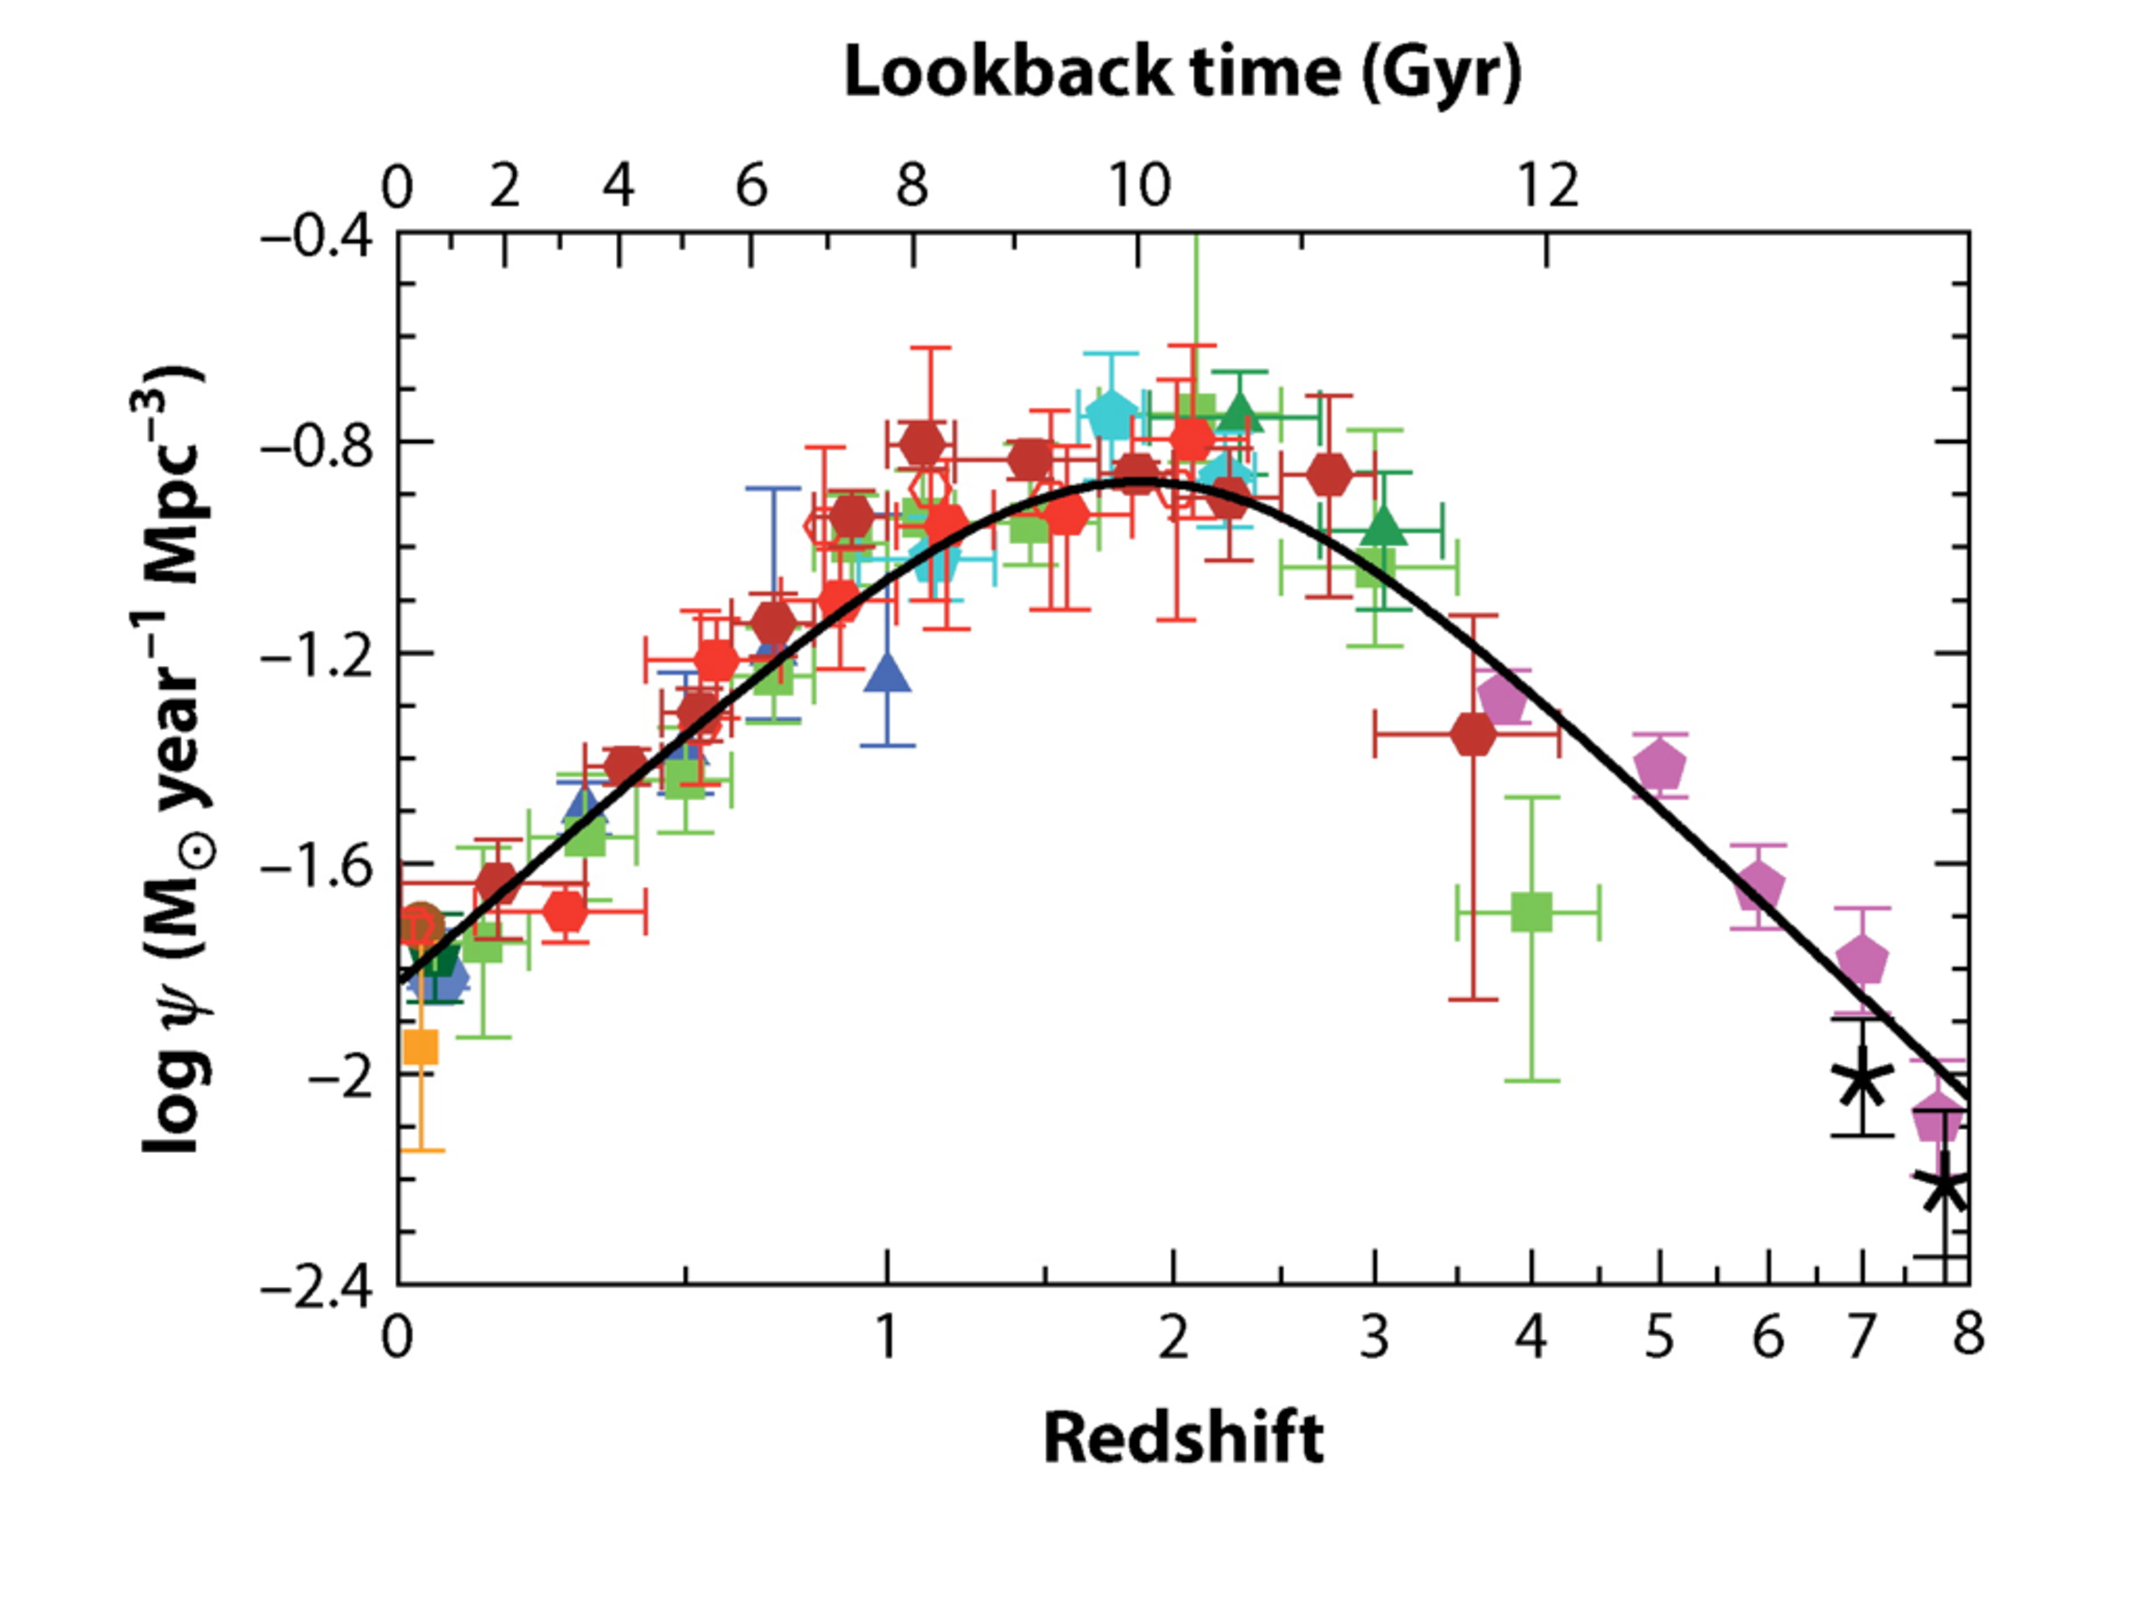
\includegraphics[width=0.5\textwidth]{madau_plot.pdf}
%  \caption{\small From Madau \& Dickinson (2014) }\label{fig:Madau_plot}
% \end{wrapfigure}

%A critical transition in evolution of galaxies in our Universe emerges
%when one considers the volumetric star-formation rate as a function of
%cosmic time 
%
% - cosmic star-formation rate shows the unique phases of the growth of
% galaxies in the Universe
%
% - the detailed cause for the decline in the CSFR since z~2 remains
% unclear, but it could be thought of as the starvation of galaxies from
% the rapid gas accretion they enjoyed in the early universe.
%
% - the outbreak of star-formation sparked by free-falling accretion of
% gas is now stymied by the size of the galaxies themselves.
%
% - a number of fundamental properties of galaxies have emerged over the
% past ~30 years: mass, size, metallicity, star-formation rate, angular
% momentum, and gas fraction.  Environment
%
%
%The rate at which stars have been born in the Universe has varied
%dramatically over cosmic history.  At roughly half its current age, the
%Universe was on average forming 10 stars for every one star formed
%today \comment{ref}.  At these epochs, galaxies looked rather different
%then they do now, dominated by all-consuming star-formation regions
%\comment{ref}.  These morphologies are only seen in rare star-burst
%galaxies in the Local Volume \comment{ref}.  The 



\subsubsection{Unraveling the Formation History of our Local Group of Galaxies}
\label{sec:localgroup}
\noindent \comment{1 page}

While only a single realization of the galaxy-formation process, our
Local Group provide unparalleled opportunities to study galaxies in
exquisite detail, by virtue of being able to spatially resolve their
constituent parts.  In fact, the Gaia satellite (ref) is currently
revolutionizing our understanding of our Milky Way Galaxy, providing
distances and on-sky motions for more than a billion stars spanning the
full extent of its disk.  These data represent a gigantic leap forward
in our ability to construct a history of the Milky Way by effectively
tracing its stellar populations and dynamical structures back in time.
However, the Gaia data are still limited: Fewer than 10\% of stars will
have a full complement of three-dimensional space motions, fewer than
0.3\% will have the basic stellar parameter measurements needed to
classify the stellar type, and only 0.1\% will have measured chemical
abundances.  Existing and ongoing surveys, like SEGUE, RAVE, and APOGEE,
and planned surveys, like WEAVE and 4MOST (refs), provide critical
supplementary observations, but these efforts only just begin to fulfill
the potential of the Gaia astrometric data.  Directly observing the all
1.7 billion stars is simply untenable for the foreseeable future.

Instead, a growing number of studies aim to infer the necessary
measurements using novel applications of machine-learning.  For example,
Ness et al.\ have developed {\it The Cannon}, a supervised learning
algorithm that uses spectra with known stellar parameters to label
spectra where those parameters are unknown.  In one application, they
determined three fundamental parameters for 55000 APOGEE spectra using a
1\% training sample.  Additionally, Ting et al.\ have developed {\it The
Payne}, which uses a neural network and theoretical stellar spectra to
determine 25 stellar labels.  In both of these applications, careful
attention has to be given to the limitations of the training sample,
similar to the SOM example provided in Figure 1.  At their core,
machine-learning algorithms, particularly supervised learning, are only
as good as the parameter space spanned by their training sets.

\medskip \noindent {\bf Data Science Challenge 5: Stellar parameter
determinations for a billion stellar spectra.}  To realize the full
potential of the Gaia astrometric catalog, one needs the full 6D phase
space for each star and its chemical abundance pattern.  Although
anything more than simple total metallicity measurements are out of
reach for FOBOS, a strategically developed training set observed at high
S/N can be used for kinematics and simple stellar parameter
determination.

% \medskip \noindent {\bf Data Science Challenge 6: Intelligent target
% allocation schemes that allow for the integration of high target
% density programs (such as discussed in Section X) with low density
% programs, such as this one, to appropriately meet the needs of both
% surveys.} See Section X.

% Beyond its internal chemodynamical history, LSST will also reveal
% hundreds of faint Milky Way satellites, as well as discover new
% satellites of the Andromeda and Triangulum galaxies, extending the
% census of these galaxies.  These faint galaxies provide critical tests
% of the hierarchical formation of the Local Group.

% \medskip \noindent {\bf Data Science Challenge 7: Dynamics of newly
% discovered Ultra-Faint dwarfs.}

\subsubsection{Time Domain}
\label{sec:timedomain}
\noindent \comment{1/2 page}



\section{Project Implementation}
\label{sec:project}

This proposal supports design work from November 2019 through September 2021 on the Keck-FOBOS instrumentation and the
interface between the instrument design and the envisioned FOBOS Public Survey plan, associated operational modes,
advanced data analysis tools, and final data products.  Design work on the complete package of hardware, software, and
data product deliverables is necessary to maximize the science return of the FOBOS Project.  Having advanced each of
these key components through preliminary design, we will request NSF MSRI-2 funding in 2021 to build and deploy the
instrumentation at the telescope, carry out the survey, and publicly serve the data products.  FOBOS would see first
light in 2025 and carry a total cost of \$32M (without contingency in 2019 dollars).  While we focus the current
request on work required for the preliminary design phase, we outline the overall project plan and final deliverables
in order to motivate this work.

\subsection{Keck-FOBOS Instrument Concept}
\label{sec:concept}
\noindent \comment{1 page}

\begin{figure}[h!]
 \vskip -0.1in
 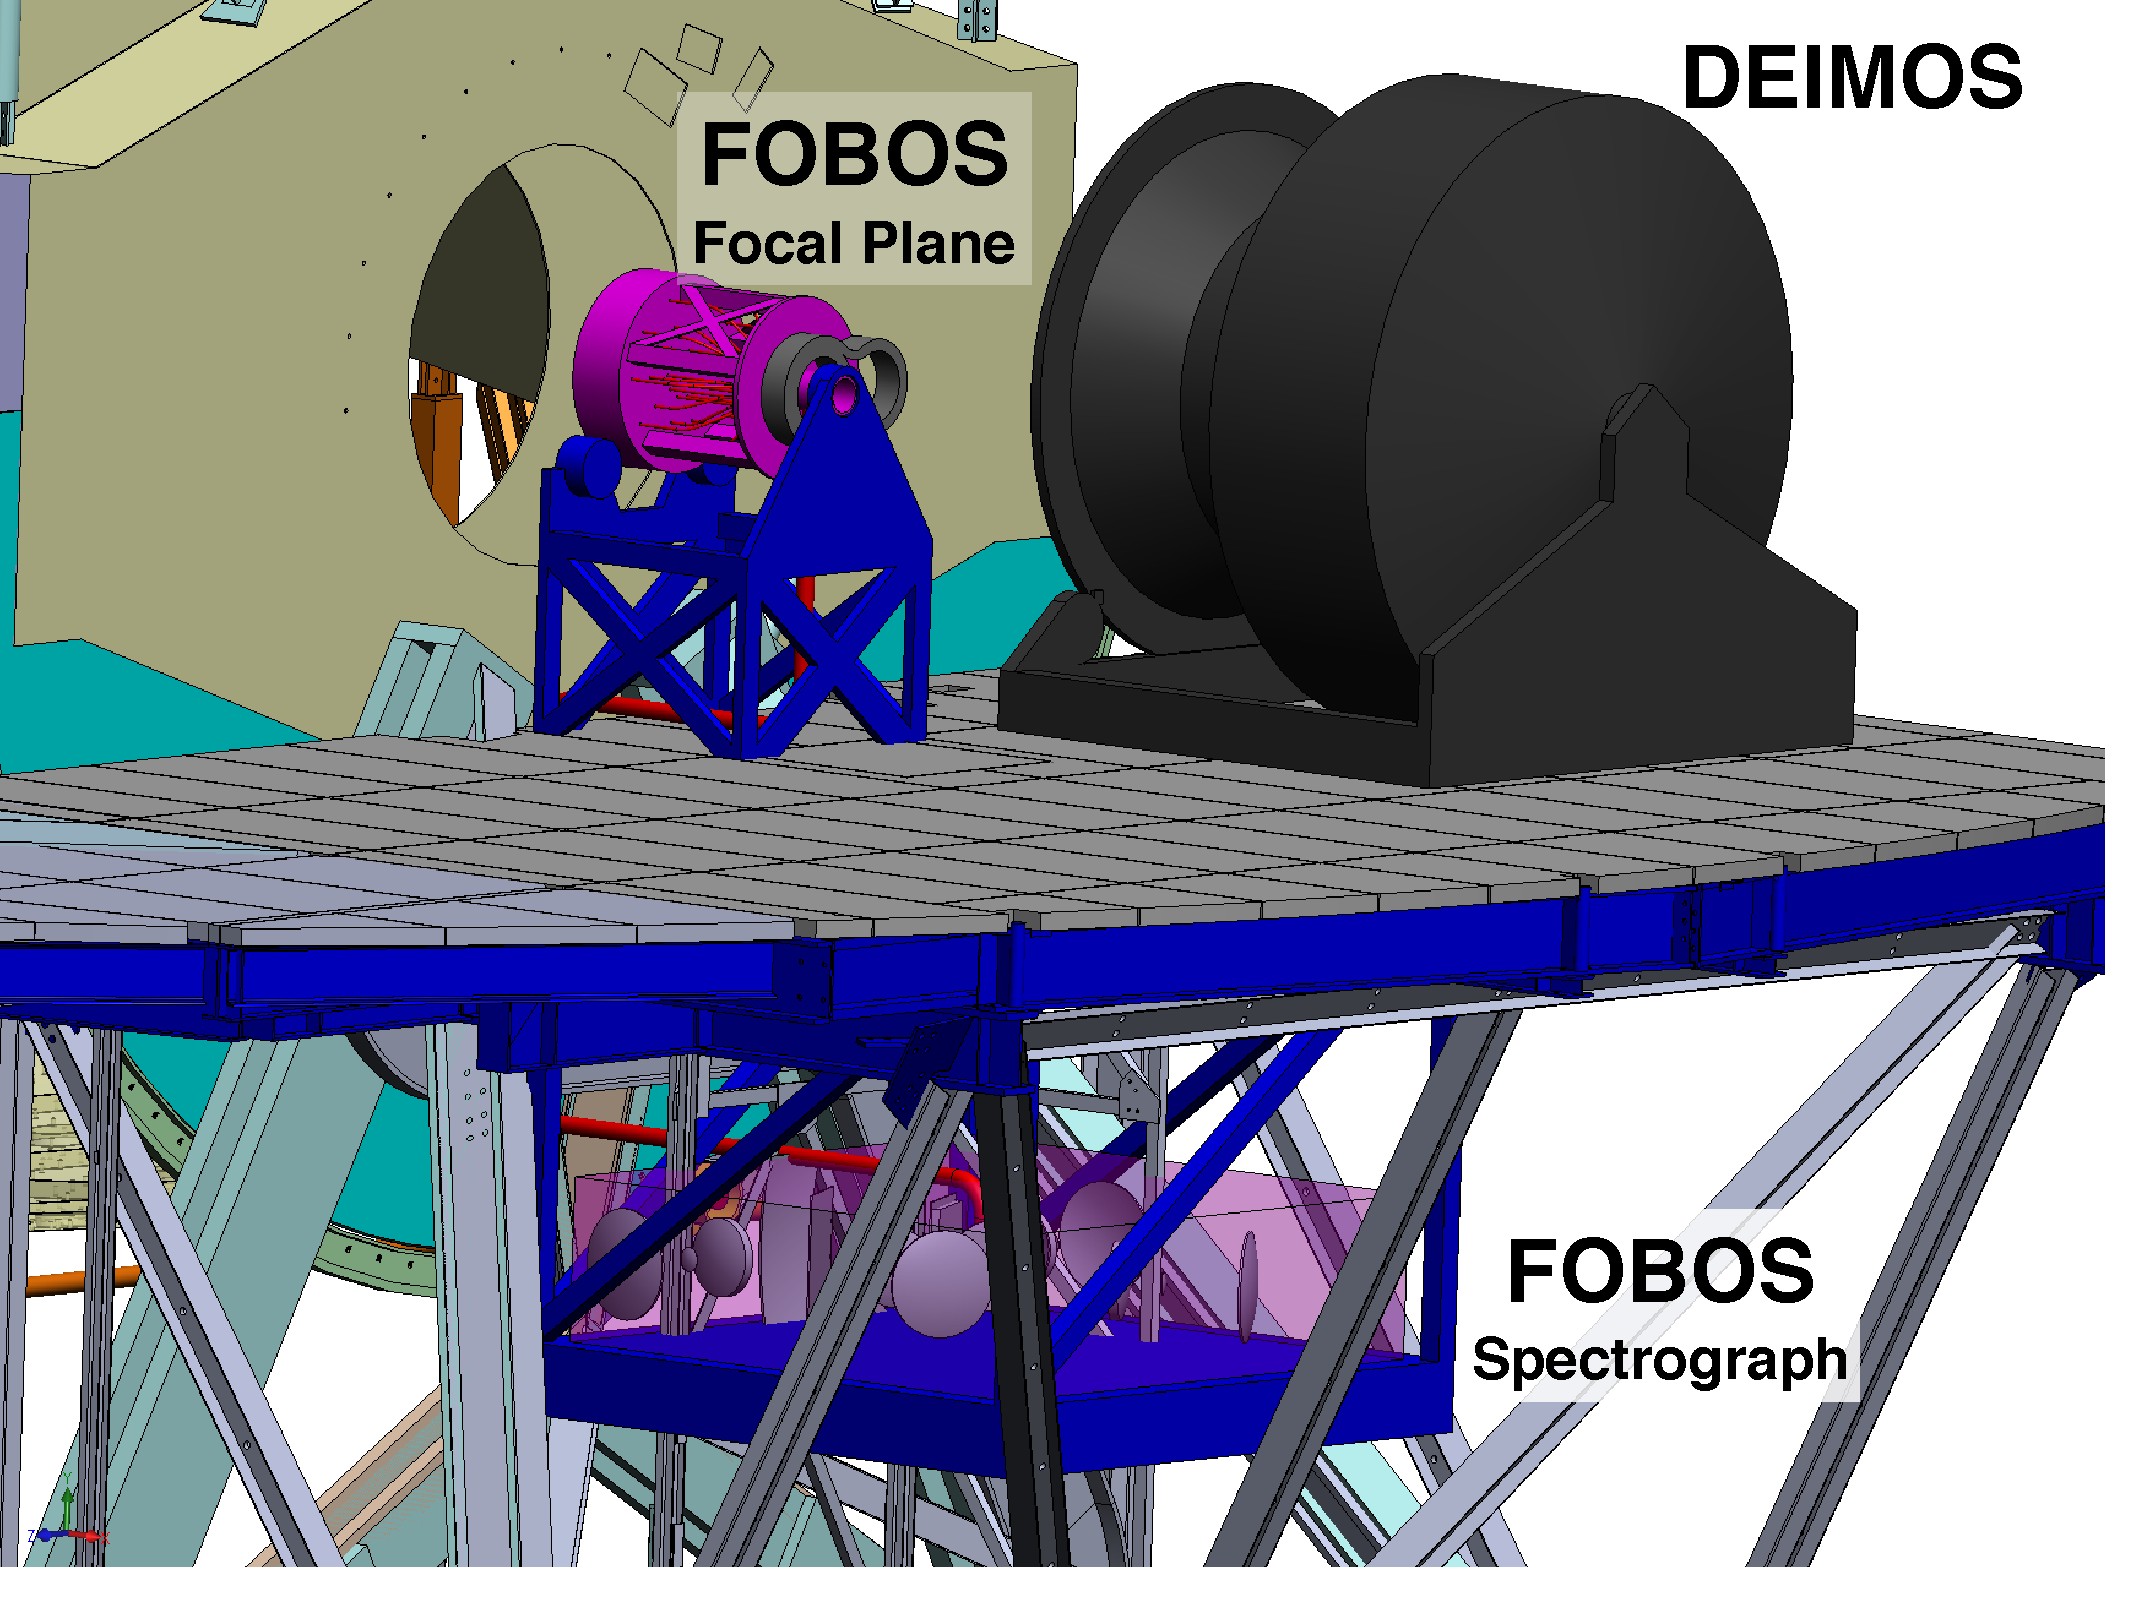
\includegraphics[width=\textwidth]{FOBOSatKeck_v1.pdf}
 \caption{\small Rendering of FOBOS instrument systems deployed at the Keck II Nasmyth port.  By mounting the FOBOS spectrographs under the Nasmyth platform, other instruments like DEIMOS can maintain access to the telescope.}\label{fig:layout}
\end{figure}

Mounted at the Keck II Telescope's Nasmyth focus, the Fiber Optic Broadband Optical Spectrograph (FOBOS) will be one of
the most powerful spectroscopic facilities in the next decade.  FOBOS consists of several key components (Fig).  A
compensating lateral atmospheric dispersion corrector (CLADC) ensures that target light from all wavelengths falls on
allocated fibers while also correcting image aberrations at the edges of the 20 arcmin diameter Keck field that result
from the telescope design.  The final lens surface in the 3-lens CLADC also serves as the mounting plate for roaming
Starbugs fiber positioners.  Starbugs patrol a large on-sky area, enabling flexible targeting configurations that can
be dynamically adjusted during observations.

A total of 1800 150 $\mu$m core diameter fibers are deployed at the curved focal plane, which rotates and translates to
maintain image positions as the telescope tracks across the sky.  The fiber run is kept at less than $\sim$10 m to
maintain high throughput at UV wavelengths, and special care is given to stress-relief cabling to minimize variable
focal ratio degradation over the fiber run.

Sets of 600 fibers feed each of three identical spectrographs.  Each spectrograph uses a series of dichroics to divide
the fiber output into four wavelength channels with combined coverage from 310 to 1000 nm and mid-channel spectral
resolutions of $R \sim 3500$.  The dispersed light in each channel is focused by an f/1.1 catadioptric camera and
recorded by an on-axis CCD mounted at the center of the first camera lens element.  Spectrographs are mounted in a
temperature controlled housing installed under the Nasmyth Deck to allow space for other Keck instruments to access the
Nasmyth port.  The end-to-end instrument throughput is greater than 30\% at all wavelengths.

FOBOS includes observatory level systems for precise instrument calibration using dome-interior screen illumination, a
metrology system for accurate fiber positioning, and guide cameras for field acquisition and guiding.  The instrument
design envisions future upgrades including alternate collecting modes that deploy multiple fiber bundles, feeds to
other fiber-based spectrographs at different wavelengths or spectral resolutions, and the ability to support and
benefit from image corrections with Ground-Layer Adaptive Optics.



\subsection{Keck-FOBOS Instrument Design Effort}
\label{sec:design}
\noindent \comment{1 page}

Keck-FOBOS will complete its current conceptual design phase in October 2019.  Funding from this proposal will support preliminary design beginning in November 2019.  A detailed schedule of activities is attached.  Major components of the preliminary design effort are described below.

\noindent \textbf{Atmospheric Dispersion Compensator (ADC).} The opto-mechanical design, tolerancing, lens cell design, motion systems, and software controls design of the ADC will be completed.  We will complete a competitive bid selection of optics vendors so that upon passing the the FOBOS Preliminary Design Review (PDR), large lens procurement can begin immediately.  This procurement is a long-lead item in the overall schedule.

\noindent \textbf{Focal Plane System.} The final ADC lens element serves as the focal plane mounting plate for the fiber positioners.  This focal plane system must rotate and translate to track the field and refraction angles from the ADC.  Mechanical design, including flexure analysis and the selection of drive mechanisms and vendors will be completed.  This system also defines one of the interfaces to the Keck Telescope and must comply with Keck Observatory space envelopes, servicing needs, and other requirements.  The focal plane system also interfaces with guide cameras for field acquisition and guiding.

\noindent \textbf{Starbugs fiber positionsers.} Starbugs are a positioning technology developed and deployed by the
Australian Astronomical Observatory (AAO) which has partnered with our team to generate a conceptual design for
Starbugs in the context of FOBOS.  Design requirements for Starbugs in FOBOS are more relaxed than the currently on-sky
TAIPAN instrument thanks to the larger physical plate scale at Keck.  AAO will serve as a vendor during preliminary
design but is interested in exploring a partnership and in-kind contribution model in the construction phase.  In addition to the Starbugs themselves, a fiber metrology system (for accurate closed-loop positioning) will also be developed.

\noindent \textbf{Fiber System.} We will complete the optical design and processing plan for affixing forward optics
lenses to each fiber's head (these demagnify and speed up the beam for proper fiber coupling).  A micro-lens array
solution will be developed for a central, fixed-position 4.5-arcsec diameter IFU for fast source acquisition.  With vendors selected, we will be ready to begin prototyping.  We will
research anti-reflective coating vendors and options and detail throughput and stress performance specifications.  This
workpackage also includes the stress-relief cable system and fiber termination hardware and processing.

\noindent \textbf{Spectrographs.} The optical systems and components (slit, collimator, dichroics, gratings, and camera), an analysis of acceptable tolerances and performance, their mechanical supports, software controls, and the overall enclosure will all be advanced through preliminary design.  Vendors for major components will complete competitive bids.  Detectors, cryostats, read-out electronics and systems for thermal management will be designed and associated vendor relationships secured. We will complete a preliminary assembly and integration plan.

\noindent \textbf{Calibration System.} This package includes design of an interior dome screen and projection system for injecting calibration sources with sufficient spatial uniformity and stability into the instrument.  We will work with the Observatory to develop an integration and controls plan.  No such calibration system currently exists at Keck.

\noindent \textbf{Auxiliary Systems.} Design of auxiliary systems includes Nasmyth platform interfaces, utilities access, fiber routing and support, thermal control and vibration control systems.


\subsection{Design of Public Survey and Training Sets}
\label{sec:survey}
\noindent \comment{1 page}

% The components of the FPS are as follows:
%     - Photo-z training samples (Newman, Masters)
%         - z>1.5 in the blue
%         - z<1.5 in the red
%     - Ly continuum
%         - z~2 in the blue
%         - z~7 in the red
%     - Machine-learning the SDSS but at z~2


\subsection{Target Allocation with Artificial Intelligence}
\label{sec:targeting}
\noindent \comment{1/2 page}


Afforded the flexibility of the Starbugs positioning system, we envision
a target allocation package that
    - maintains a database with observational progress on individual
      targets in the survey and
    - dynamically reallocates fibers based on real-time assessments of
      the aggregate S/N of each target to meet the specific need of each
      science case.

This requires significant design and testing of a combined software
package and hardware interface.  Specific considerations involve (1)
fast and robust reduction procedures (cf. MaNGA DOS) that can assess the
aggregate data and (2) a responsive database with a schema optimized for
real-time decision making to select targets for (re)acquisition while
accounting for collision limitations.  Provided enough design effort,
this lends itself to a machine-learning application.


\subsection{Pulicly Available Automated Data Products}
\label{sec:DAP}
\noindent \comment{1/2 page}

The advanced products of the survey will be delivered to the public via
the Keck Observatory Archive (KOA).  However, beyond the raw data, the
survey will provide reduced and derived products immediately (cf. MaNGA
DAP).  The latter will be true of both the data from the public survey
(released immediately) and indeed {\it any} data taken with the FOBOS
instrument after the nominal 18-month proprietary period.  For the
latter, we will encourage involvement of the program PI in refining the
data-reduction and data-analysis software and its execution to garner
the most from its application to their data.  Community involvement in a
common software development obviates the need for different groups to
retread old ground.



\section{Broader Impacts}
\label{sec:bi}

"include a discussion of student training, increased participation of
underrepresented groups and a description of tangible benefits to the
wider U.S. research community (access, data products, technology,
etc.)."

\subsection{Student training}
\label{sec:training}
\noindent \comment{1/4 page}

\subsection{ISEE?}
\noindent \comment{1/2 page}

% AKAMAI: local Hawaiian workforce
%     - many more computer science students
%         UH Hilo 
%     - UH manao mostly engineering

%     - AMOS - airforce 
%         - abstract
% 
% 
%     1/3 of students on mainland but from hawaii
% 
%     1/4 are native hawaii
% 
%     38\% women
% 
%         \$15k intern
% 
%         2 students for 2 summers?
% 
%     4/5 day prep for prof dev
% 
% Prof dev program:
%     grads postdocs
%         - learn diverse students and inclusively
%         - form a team, design something, and teach it
%         - ~25 teams every year.
%         - teams geared toward specific need of ugrad groups
% 
%     chapters throughout country
%         - REU prep
%         - stats
%         - cfa summerschool
%         - dunlap summer school
% 
%         - kappa w/ Jessica Lu : astrotech
% 
%         - 
% 
%     grad+postdoc: local ~\$3500 per


\subsection{Data Science Major in Astrophysics}
\noindent \comment{1/4 page}


"Preliminary proposals must include an outline of ongoing operations and
maintenance plans, including an estimate of any needs for ongoing,
NSF-supported operations and maintenance that may be requested outside
of the Mid-scale RI program."

"Results from Prior NSF Support should not be included. Also, links to
URLs may not be used."

\vspace{-0.5cm}

{\bf no more than 2 pages for references}

\clearpage
\bibliographystyle{nsf}
\bibliography{references}


\newpage

\noindent{\bf Budget and Budget Justification}

"including budgets for any subawards. For preliminary proposals cost
estimates may be preliminary estimates with the Basis of Estimates (BoE)
included. Copies of vendor quotations should not be included in
preliminary proposals. If the budget includes contingency, that
contingency should cover the "known unknowns" and be used to mitigate
identified risks."

\newpage

\noindent{\bf Facilities, Equipment, and Other Resources:}

In order for NSF, and its reviewers, to assess the scope of a proposed
project, all organizational resources necessary for, and available to a
project, must be described in this section of the proposal. Proposers
should describe only those resources that are directly applicable. The
description should be narrative in nature and must not include any
quantifiable financial information. Proposers should include a
description of the internal and external resources (both physical and
personnel) that are expected to be available to the project.  Such
information must be provided in this section, in lieu of other parts of
the proposal (e.g., Budget Justification, Project Description).

\newpage

\noindent{\bf Supplementary Documents:}

(to be entered in the Supplementary Documents section of FastLane)

\begin{enumerate}
%
\item A list of the major team members, their affiliations, and their
role in the project;
%
\item A list of Partner Organizations to be funded via subawards, and
the role of each in the project;
%
\item An outline of the Project Execution Plan (PEP).
%  see https://www.nsf.gov/bfa/lfo/lfo_documents.jsp
\end{enumerate}

(See the LFM/MFG. Greater detail will be required in invited full
proposals should that occur. See Full Proposal Preparation section for
further information.)

%\begin{figure}[h!]
%  \vskip -0.1in
%  \includegraphics[width=\textwidth]{red_geyser_fig.pdf}
%  \caption{\small Discovery of the ``red geyser'' phenomenon in MaNGA which may
%      provide key missing evidence for how early-type galaxies remain quiescent.  Our prototypical example is the
%      elliptical galaxy (MaNGA ID 1-217022) pictured to the right in the SDSS image (top panel) and tidally interacting
%      with a low-mass companion.  The purple hexagons show the MaNGA integral-field footprint.  Bisymmetric features in
%      the H$\alpha$ equivalent width map (EW, central panel) suggest outflowing material.  A cool gas component traced
%      by Na D is offset, however, with material apparently falling into the galaxy's center (center-right panels).
%      Further evidence for an outflowing ionized gas is apparent emission line velocity field ($v_{\rm gas}$,
%      bottom-center panel).  Schematic diagrams of a wind model are shown to the left while the bottom-right panel
%      demonstrates how features in the $v_{\rm gas}$ field can be reproduced by the model.  The enhanced H$\alpha$
%      emission (over-plotted white contours) can be explained by shocks or over-densities occurring along the central
%      wind axis (highlighted in green in the wind drawings).  Other examples of MaNGA red geysers are shown in Figure
%      \ref{fig:montage}. }\label{fig:splash}
%\end{figure}


% \begin{enumerate}[rightmargin=0.2cm,leftmargin=0.2cm]
%
%  \item[] {\bf Preparatory Work}: Using a parent sample of 2400 MaNGA galaxies we apply a red sequence color cut of
%  $NUV-r>5$ \citep[see][]{salim09} which yields $\sim$1000 quiescent galaxies from which we visually identify 83 red
%  geyser candidates.  We have built a control sample of 442 galaxies by matching on redshift, $M_*$, and axis ratio
%  ($b/a$).  Stellar mass and redshift have been shown to correlate with radio emission and thus must be controlled for
%  \citep[e.g.,] []{best07}.  We additionally consider a control sub-sample with MaNGA-detected emission lines (LIER
%  galaxies).
%
%  We have downloaded FIRST radio image data and extracted cutouts centered on both the red geyser and control samples.
%   Among these we have identified radio detections and performed initial median stacks which are shown in Figure
%   \ref{fig:stacks}.  We find that 19/83 ($\approx23\%$) red geysers and 39/442 ($\approx9\%$) control galaxies are
%   radio-detected.  Our prelminary stacked photometry indicates that with detections removed, the radio flux associated
%   with red geysers is $\approx$7 times stronger than in the control samples.
%
%  \item[] {\bf Proposed Work}: Our preliminary analysis of the FIRST data points to an important result: radio
%  emission, most likely associated with AGN, appears to be elevated among red geysers bolstering our AGN wind
%  interpretation.  Here we propose to complete and publish this analysis.  We will update the red geyser sample using
%  the latest MaNGA catalog ($\sim$5000 galaxies, see Section \ref{sec:stats}) and more carefully vet the stacked
%  samples.  Using deep star formation rate estimates from \citet{chang15}, we will test that radio flux
%  contamination from residual star formation does not affect our conclusions.  Most important, we will develop a Monte
%  Carlo technique to measure the photometric errors on our stacked flux estimates.  This will enable us to assign a
%  confidence level to the significance of the stronger radio flux associated with red geysers.  
%

%\end{enumerate}


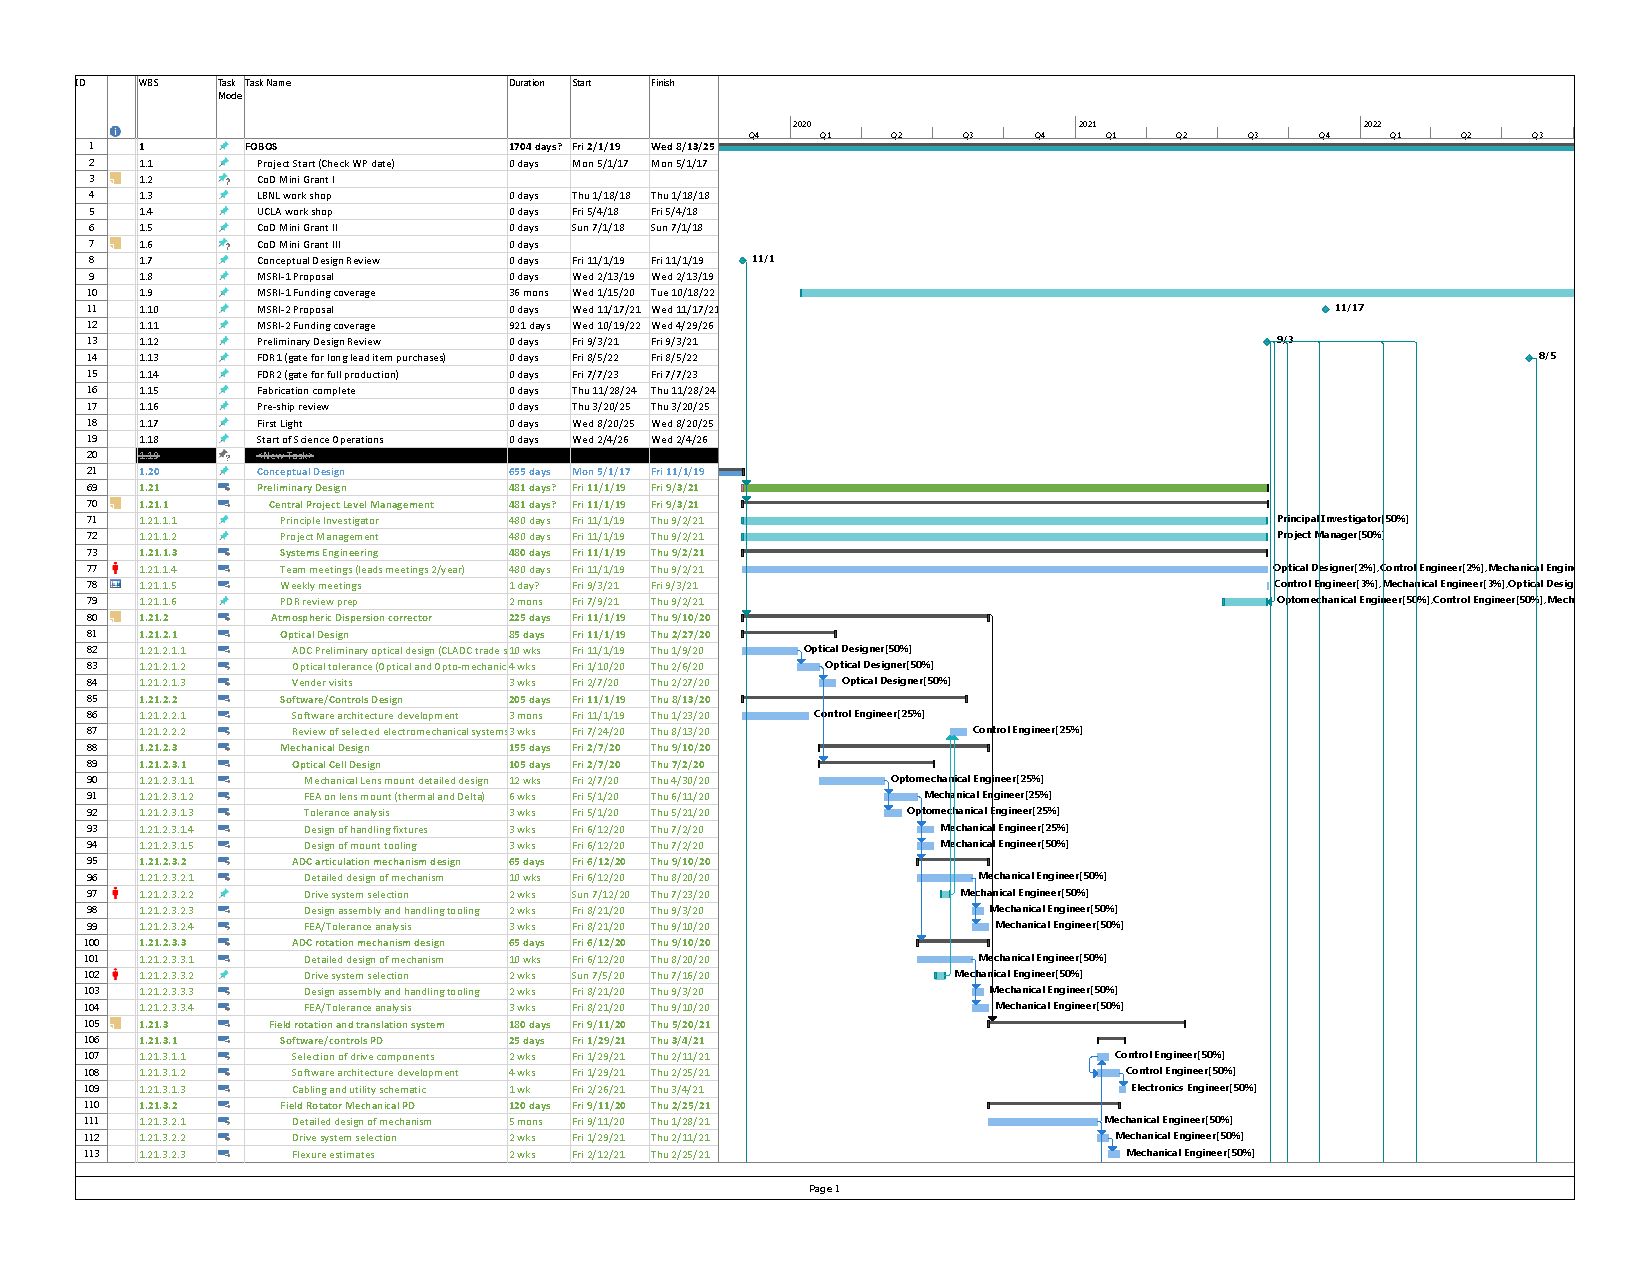
\includepdf[pages=-,landscape=true]{FOBOS_HighLevel_Schedule_v1.pdf}

\end{document}

